\documentclass{article}
\usepackage{amssymb}
\usepackage{amsmath}
\usepackage{mathtools}
\usepackage{cancel}
\usepackage{tikz}
\usepackage{hyperref}
\usepackage{circuitikz}
\usepackage{float}
\usepackage{afterpage}
\usepackage{listings}
\usepackage{caption}
\usetikzlibrary{calc, shapes.gates.logic.US, positioning}
\newtheorem{theorem}{Theorem}
\newtheorem{definition}{Definition}
\newtheorem{corollary}{Corollary}
\newtheorem{proof}{Proof}

\DeclareMathOperator*{\argmin}{argmin}

\begin{document}
\title{CS61C Course Notes}
\author{Anmol Parande}
\date{Fall 2019 - Professors Dan Garcia and Miki Lustig}
\maketitle
\tableofcontents
\newpage
\textbf{Disclaimer: }These notes reflect 61C when I took the course (Fall 2019). They may not accurately reflect current course content, so use at your own risk.
If you find any typos, errors, etc, please report them on the \href{https://github.com/parandea17/BerkeleyNotes}{GitHub repository}.
\section{Binary Representation}
Each bit of information can either be 1 or 0. As a result, $N$ bits can represent at most $2^N$ values.
\subsection{Base conversions}
\textbf{Binary to Hex conversion}
\begin{itemize}
    \item Left pad the number with 0's to make 4 bit groups
    \item Convert each group its appropriate hex representation
\end{itemize}
\textbf{Hex to Binary Conversion}
\begin{itemize}
    \item Expand each digit to its binary representation
    \item Drop any leading zeros
\end{itemize}
\subsection{Numeric Representations}
When binary bit patterns are used to represent numbers, there are nuances to how the resulting representations are used.
\begin{definition}
    Unsigned integers are decimal integers directly converted into binary. They cannot be negative.
\end{definition}
\begin{definition}
    Signed integers are decimal integers whose representation in binary contains information denoting negative numbers.
\end{definition}
Binary math follows the same algorithms as decimal math. However, because computers only have a finite number of bits
allocated to each number, if an operation's result exceeds the number of allocated bits, the leftmost bits are lost.
This is called \textbf{overflow}
\subsubsection{Sign and Magnitude}
In the sign and magnitude representation, the leftmost bit is the sign bit.
A 1 means the number is negative where as 0 means it is positive. The downside to this is when overflow occurs, adding one does not wrap the bits properly.
\subsubsection{One's Complement}
To fix the bit wrapping, to form the negative number, we can flip each bit. This solves the wrapping issue so even with overflow, when adding 1, the result will continue increasing.
\subsubsection{Two's Complement}
To convert from decimal to two's complement:
If the number is positive, convert to binary as normal.
If the number is Negative:
\begin{itemize}
    \item[1.] Convert the positive version of the number to binary
    \item[2.] Invert each bit
    \item[3.] Add one to the result
\end{itemize}
If given a two's complement number, you can find -1 times that number by following the same process (invert bits and add 1).
\subsubsection{Bias Encoding}
With bias encoding, the number is equal to its unsigned representation plus a bias turn. With a negative bias,
we can center a positive range of $0 \rightarrow 2^N - 1$ on 0.
\subsection{Floating Point Representation}
To represent decimal numbers in binary, we use floating point representation.
Any number in scientific notation has the following components
\begin{itemize}
    \item Mantissa: The number in front of the point
    \item Significand: The digits after the point
    \item Radix: The base of the number
    \item Exponent: How many times the point should be shifted to recover the original number
\end{itemize}
\[
    \underbrace{1}_{\text{Mantissa}}\underbrace{.}_{\text{Binary Point}}\underbrace{01}_{\text{significand}} \cdot \underbrace{2 ^ {\overbrace{-1}^{\text{exponent}}}}_{\text{radix}} 
\]
If we have a 32 bit system, then by the floating point convention:
\[
    \underbrace{0}_{\text{Sign Bit}}\overbrace{00000000}^{\text{Exponent Bits}}\underbrace{00000000000000000000000}^{\text{Significand}}
\]
In the floating point representation, the manissa is always one because we are using scientific notation, so we don't bother storing it.
\begin{itemize}
    \item Sign Bit: Determines the sign of the floating point number
    \item Exponent: 8 bit biased number (-127 bias)
    \item Significand: 23 significand bits representing $2^{-1}, 2^{-2}...$
\end{itemize}
Given a number in floating point representation, we can convert it back to decimal by applying the following formula:
$$n = (-1)^s(1+significand)\cdot2^{exponent - 127}$$
Notice a couple things about this representation.
\begin{itemize}
    \item If the exponent is larger than 8 bits, then overflow will occur
    \item If a negative exponent is more than 8 bits, then underflow occurs
    \item There are 2 0's. Positive 0 and negative 0
\end{itemize}
Because of the way that floating point is built, certain sequences are designated to be specific numbers
\begin{center}
    \begin{tabular}{c|c|c}
     Exponent & Significand & Object \\
     \hline
     0 & 0 & 0 \\  
     0 & nonzero & denorm\\
     1-254 & anything & $\pm$ \#\\
     255 & 0 & $\pm \infty$\\
     255 & nonzero & NaN    
    \end{tabular}
\end{center}
A \textbf{denormed number} is a number where we don't have an implicit 1 as the mantissa. These
numbers let us represent incredibly small numbers. They have an implicit exponent of $-126$.
\section{C}
\subsection{C Features}
\begin{itemize}
    \item C is a compiled language $\implies$ executables are rebuilt for each new system
    \item Every variable holds garbage until initialization
    \item Function parameters are pass by value
\end{itemize}
\subsection{Bitwise Operators}
Bitwise operators are operators which change the bits of integer-like objects (ints, chars, etc)
\begin{itemize}
    \item $\&$: Bitwise AND. Useful for creating masks
    \item $|$: Bitwise OR. Useful for flipping bits on
    \item $\wedge$: Bitwise XOR. Useful for flipping bits off
    \item $<<$: Left shifts the bits of the first operand left by the number of bits specified by the second operand.
    \item $>>$: Right shifts the bits of the first operand right by the number of bits specified by the second operand.
    \item $\sim$: Inverts the bits.
\end{itemize}
\subsection{Pointers}
\begin{definition}
    The address of an object is its location in memory
\end{definition}
\begin{definition}
    A pointer is a variable whose value is the address of an object in memory
\end{definition}
\subsubsection{Pointer Operators}
\begin{itemize}
    \item $\&$: Get the address of a variable
    \item $*$: Get the value pointed to by a pointer
\end{itemize}
Because C is pass by value, pointers allow us to pass around objects without having them copied.
They can also lead to cleaner, more compact code. However, always remember that declaring a pointer
creates space for an object but \textbf{does not} put anything in that space (i.e it will be garbage).\\\\
Pointers can point to anything, even other points. For example, $int **a$ is a pointer to an integer pointer. 
This is called a handle
\subsection{Arrays}
In C, arrays are represented as adjacent blocks of memory. The way that we interact with them is through pointers.
Consider
\begin{lstlisting}[language=C]
    int a[];
    int *b;
\end{lstlisting}
Both of these variables represent arrays in C. They point to the first memory location of the array.
C arrays can be indexed into using [] subscripts like other programming languages. They can also be
index into using pointer arithmatic. For example, $*(a+2) \equiv a[2]$. By adding 2 to a, C knows to 
look two memory locations into the array (i.e the third element).\\\\
C is able to do this because it automatically computes the size of the objects in the array to know how
much to advance the pointer by.
\begin{lstlisting}[language=C]
    int a[] = {1, 2, 3, 4, 5}; //ints are 4 bytes;
    printf("%u", &a); // 0x2000
    printf("%u", &(a+2)); // 0x2008
    char *c = "abcdef"; //chars are 1 byte
    printf("%u", &c); // 0x3000
    printf("%u", &(a+c)); // 0x3002
\end{lstlisting}
One important thing to remember is that declared arrays are only allocated while the scope is valid.
That means once a function returns, their memory is free to be taken.\\\\
Another important consideration in C is that C arrays do not know their own lengths and they do not check their bounds.
This means whenever you are passing an array to a function, you should always be passing its size as well.
\subsection{Structs}
Structs are the basic datastructures in C. Like classes, they are composed of simpler data structures,
but there is no inheritance.
\subsubsection{Struct Operators}
\begin{itemize}
    \item $->$: dereference a struct and get a subfield
\end{itemize}
$typedef$ can be a useful command with structs because it lets us name them cleanly.
\section{Memory Management}
\subsection{Memory Basics}
In memory, a \textbf{word} is 4 bytes. When objects are saved to memory, they are saved by words. How the words are ordered depends on the type of system.
In \textbf{Little Endian} systems, the Least Significant Byte is placed at the lowest memory address. In other words, the memory address points to the least significant byte\\\\
The opposite is true in \textbf{Big Endian} systems.
For example, lets say we have the number $0x12345678$ stored at the memory address $0x00$
\begin{center}
    \begin{tabular}{c|c|c|c|c}
        & $0x00$ & $0x04$ & $0x08$ & $0x0C$\\
        \hline
        Little Endian: & 78 & 56 & 34 & 12\\
        \hline
        Big Endian: & 12 & 34 & 56 & 78
    \end{tabular}
\end{center}
There are four sections of memory: the stack, the heap, static, and code. 
\begin{definition}
    The Stack is where local variables are stored. This includes parameters and return addresses. It is the "highest" level of memory and grows "downward" towards heap memory.
\end{definition}
\begin{definition}
    The Heap is where dynamic memory is stored. Data lives here until the programmer deallocates it. It sits below the stack and grows upwards to toward it.
\end{definition}
\begin{definition}
    Static storage is where global variables are stored. This storage does not change sizes and is mostly permanent.
\end{definition}
\begin{definition}
    Code storage is where the "code" is located. This includes preprocessing instructions and function calls.
\end{definition}
\begin{definition}
    Stackoverflow is when the stack grows so large that it intersects with heap memory. This is mostly unavoidable.
\end{definition}
\begin{definition}
    Heap pileup is when the heap grows so large that it starts to intersect with the stack. This is very avoidable because the programmer manages it.
\end{definition}
\begin{definition}
    All of the memory which a program uses is collectively referred to as the address space of the program.
\end{definition}
\subsection{The Stack}
The stack is named that way because every time a function call is made, a stack frame is created.
A stack frame includes the address of the return instruction and the parameters to the function. As the function executes,
local variables are added to the frame. When the function returns, the frame is popped off. In this way, frames are handled in 
Last-In-First-Out (LIFO) order.
\begin{definition}
    The stack pointer is a pointer which points to the current stack frame.
\end{definition} 
\textbf{Important: }Deallocated memory is not cleared. It is merely overwritten later.
\subsection{The Heap}
The heap is a larger pool of memory than the stack and it is not in contiguous order. Back to back allocations to the heap may be very far apart.
\begin{definition}
    Heap fragmentation is when most of the free memory in the heap is in many small chunks
\end{definition}
Fragmentation is bad because if we want to allocate space for a large object, we may have enough cumulative space on the heap,
but if none of the remaining contiguous spaces are open, then there is no way to create our object.\\\\
\textbf{Implementation:}\\\\
Every block in the heap has a header containing its size and a pointer to the next block.
The free blocks of memory are stored as a circular linked list.
When memory needs to be allocated to the heap, this linked list is searched.
When memory is freed, adjacent empty blocks are coalesced into a single larger block.
There are three different strategies which can be used to do this allocation/freeing.
\begin{definition}
    Best-fit allocation is where the entire linked list is searched to find the smallest block large enough to fit the requirements
\end{definition}
\begin{definition}
    First-fit allocation is where the first block that is large enough to fit the requirement is returned
\end{definition}
\begin{definition}
    Next-fit allocation is like first-fit allocation except the memory manager remembers where it left off in the free list and resumes searching from there.
\end{definition}
\subsection{Heap Management}
As a C programmer, it is up to us to manage the heap memory. This is done through the $malloc$ function.
\begin{lstlisting}[language=C]
    malloc(size_t size)
\end{lstlisting}
Malloc takes a size in bytes and returns a pointer to the allocated memory in the heap. If there is no space in the heap, then it returns $NULL$.
Any space created with $malloc$ must be freed using the $free$ function.\\
\textbf{Things to watch out for: }
\begin{itemize}
    \item Dangling reference (A pointer used before malloc)
    \item Memory Leak (When $free$ isn't called or the pointer is lost but $free$ wasn't called)
    \item Do not free the same memory twice
    \item Do not use free on something not created with malloc
    \item malloc does not overwrite what was in the current memory location.
\end{itemize}
Because we need to tell $malloc$ how much space we need allocated, we will often use the $sizeof$ function.
This returns the size in bytes of whatever type or object you give it. This allows us to write code for different architectures (i.e 32bit vs 64bit)
\section{RISC-V}
\subsection{Basics of Assembly Languages}
In Assembly Languages like RISC-V, instructions are executed directly by the CPU. The basic job of the CPU is to taken
a set of instructions and execute them in order. The \textbf{Instruction Set Architecture} (ISA) determines how this is done.
In \textbf{Reduced Instruction Set Computing} (RISC) languages, the instruction set is limited because it makes the hardware simple.
Complex operations are left to the software.\\\\
\textbf{Registers} are the operands of assembly language operations. A register is a memory location on the CPU itself. There are a limited
number of them, but they are very fast. In RISC-V processors, there are 32 registers. Each register can store one \textbf{word}.
This is 32 bits on a 32-bit system.\\\\
Registers are labeled x0-x31. x0 is a special register because it always holds the value 0. Unlike variables, registers have no types. The operation
is what determines what the content of the register is treated as.\\\\
\textbf{Immediates} are numerical constants. They can also be used as the operands of assembly intructions.
\subsection{RISC-V Structure}
The general format of a RISC-V instruction is
\begin{lstlisting}
    operation_name destination source1 source2
\end{lstlisting}
\textbf{Labels} are text in the program which denote certain locations in code. \textbf{Branches} change the flow of the program,
usually by jumping to a label or an address in the code portion of memory.\\\\
\textbf{Pseudo-instructions} are instructions which are translated into different instructions by the assembler. They exist because they increase
readability of the program.\\\\
In order to increase program legibility, labels are hardly referred to by their number (x15, x20, etc). Instead, they have symbolic names. Here are a few.
\begin{itemize}
    \item a0 - a7: The argument registers
    \item s0 - s7: The saved registers
    \item ra: return address register
    \item sp: stack pointer register
    \item pc: Program Counter
\end{itemize}
\subsubsection{Caller Callee Convention}
Because functions can always overwrite registers, programmers set up conventions for calling and returning from functions.
The \textbf{Caller} is the function which calls another function. The \textbf{Callee} is a function which is being called.\\\\
\textbf{Functional Control Flow}
\begin{itemize}
    \item[1.] Put paramters where the function can access them (a0-a7)
    \item[2.] Transfer control to the function (jump)
    \item[3.] Acquire the local storage resources for function (Increase stack)
    \item[4.] Perform the desired task of the function
    \item[5.] Put result in $a0$ where the calling function can access it
    \item[6.] Release local variables and return data to used registers so the caller can access them (Decrease stack)
    \item[7.] Return control to the calling function (Jump to $ra$)    
\end{itemize}
Because every function must have this control flow, the caller-callee convention was set up as follows
\begin{itemize}
    \item[1.] sp, gp, tp, s0-s11 are preserved across a function call
    \item[2.] t0-t7, a0-a7 are not preserved across a function call
\end{itemize}
If a register is not preserved across a function call, then the caller cannot expect its value to be the same
after the callee returns. In order to preserve registers across a function call, we use the \textbf{stack}. The
Stack Frame stores the variables which need to be saved in order to adhere to caller callee convention. Every RISC-V
function has a \textbf{Prologue} where it saves the neccessary registers to the stack. An example might look like
\begin{lstlisting}
    addi sp, sp, -16
    sw s0, 0(sp)
    sw s1, 4(sp)
    sw s2, 8(sp)
    sw ra, 12(sp)
\end{lstlisting}
This function must use the s0-s3 saved registers. We first create the stack frame by decrementing the stack pointer.
Then we save the saved registers to the newly allocated memory. This function must be calling another function, so it
has to remember its return address. That is why we save it to stack. The \textbf{Epilogue} is the part of the function
before it returns where everything on the stack is put back.
\begin{lstlisting}
    lw s0, 0(sp)
    lw s1, 4(sp)
    lw s2, 8(sp)
    lw ra, 12(sp)
    jr ra
\end{lstlisting}
\subsubsection{Directives}
Directives are special demarcations in an assembly file which designated different pieces of data.
\begin{itemize}
    \item[.text:] Subsequent items are put into the text segment of memory (i.e the code)
    \item[.data:] Subsequent items are put into the data segment of memory (i.e static variables)
    \item[.global sym:] Declares a symbol to be global, meaning it can be referenced from other files
    \item[.string str] Stores a null-terminated string in the data memory segment
    \item[.word] Store n 32 bit quantities into contiguous memory words.
\end{itemize}
\subsection{Instruction Formats}
In a \textbf{Stored Program Computer}, instructions are represented as bit patterns. They are stored in
memory just like data. As a result, everything has a memory address, including lines of code. The \textbf{Program Counter}
is the memory address of the current instruction. Each instruction in RISC-V is 1 word, or 32 bits.
It is divided into fields, each of which tells the processor something about the instruction.
\begin{itemize}
    \item[R Type:] Register-register arithmetic 
    \item[I Type:] Register-immediate arithmetic
    \item[S Type:] Store instructions
    \item[B Type:] Branch instructions
    \item[U Type:] 20 bit upper immediate instructions
    \item[J Type:] Jump Instructions    
\end{itemize}
Every instruction type has a 7 bit \textbf{opcode} which tells the processor what instruction type it is processing.
These are always the last 7 bits. Some instructions also have \textbf{funct3} and \textbf{funct7} fields which define
the operation to perform in conjunction with the opcode.\\\\
\textbf{R-Type}
\begin{center}
    \begin{tabular}{|c|c|c|c|c|c|}
        31:25& 24:20& 19:15& 14:12 & 11:7 & 6:0\\
        \hline
        funct7 & rs2 & rs1 & funct3 & rd & opcode\\
        \hline
    \end{tabular}
\end{center}
\textbf{I-Type}
\begin{center}
    \begin{tabular}{|c|c|c|c|c|}
        31:20& 19:15& 14:12 & 11:7 & 6:0\\
        \hline
        Imm[11:0] & rs1 & funct3 & rd & opcode\\
        \hline
    \end{tabular}
\end{center}
\textbf{S-Type}
\begin{center}
    \begin{tabular}{|c|c|c|c|c|c|}
        31:25 & 24:20 & 19:15 & 14:12 & 11:7 & 6:0\\
        \hline
        Imm[11:5] & rs2 & rs1 & funct3 & Imm[4:0] & opcode\\
        \hline
    \end{tabular}
\end{center}
\textbf{B-Type}
\begin{center}
    \begin{tabular}{|c|c|c|c|c|c|c|c|}
        31 & 30:25 & 24:20 & 19:15 & 14:12 & 11:8 & 7 & 6:0\\
        \hline
        Imm[12] & Imm[10:5] & rs2 & rs1 & funct3 & Imm[4:1] & Imm[11] & opcode\\
        \hline
    \end{tabular}
\end{center}
\textbf{U-Type}
\begin{center}
    \begin{tabular}{|c|c|c|}
        31:12 & 11:7 & 6:0\\
        \hline
        Imm[31:12] & rd & opcode\\
        \hline
    \end{tabular}
\end{center}
\textbf{J-Type}
\begin{center}
    \begin{tabular}{|c|c|c|c|c|c|}
        31 & 30:21 & 20 & 19:12 & 11:7 & 6:0\\
        \hline
        Imm[20] & Imm[10:1] & Imm[11] & Imm[19:12] & rd & opcode\\
        \hline
    \end{tabular}
\end{center}
\subsubsection{Addressing}
Notice that the J-Type and B-Type instructions require use a label in code.
These labels are encoded in the instruction format as an offset from the program counter.
This is known as \textbf{PC Relative Addressing}. Since each instruction in RISC-V is 1 word,
we will never have an odd address. As a result, we don't need to store the last bit of the immediate
in B-Type and J-Type instructions because it is automatically 0.
\subsection{Compiling, Assembling, Linking, Loading}
Compiling, Asssembling, Linking, and Loading (\textbf{CALL}) are the four steps of loading a program.
\subsubsection{Compiler}
The input to the compiler is a file written in a high level programming language. It outputs assembly language
code which is built for the machine the code was compiled on. The output of the compile may still include 
pseudo-instructions in assembly.
\subsubsection{Assembler}
The Assembler is the program which converts assembly language code to machine language code. It reads and uses
directives, replaces psuedo-instructions with their real equivalent, and produces machine language code (i.e bits)
where it can.\\\\
The output of the assembler is an object file. The object file contains the following elements:
\begin{itemize}
    \item Object file header: The Size and position of the different sections of the object files
    \item Text Segment: The code
    \item Data Segment: binary representation of the static data in the source
    \item Relocation Table: A special data structure which contains the lines of code needing to be fixed
    \item Symbol Table: A special data structure which lists the files global labels and static data labels
    \item Debugging information
\end{itemize}
The symbol table contains information which is public to other files in the program.
\begin{itemize}
    \item Global function labels
    \item Data Labels
\end{itemize}
The Relocation Table contains information that needs to be relocated in later steps. It essentially tracks
everything that the Assembler cannot directly convert to machine code immediately because it doesn't have
enough information.
\begin{itemize}
    \item List of labels this file doesn't know about
    \item List of absolute labels that are jumped took
    \item Any piece of data in the static section
\end{itemize}
% TODO: Double Check This
When the assembler parses a file, instructions which don't have a label are converted into machine language. When a label is defined,
it's position is stored in the relocation table. When a label is encountered in code, the assembler looks to see if it's position
was defined in the relocation table. If it is found, the label is replaced with the immediate and converted to machine code.
Otherwise, the line is marked for relocation.\\\\
In order to do its job, the assembler must take two passes through the code. This is because of the \textbf{forward reference problem}.
If a label is used before it is defined in the same file, the first time the assembler encounters it, it won't know how to convert it to machine code.
To resolve this, the assembler simply takes two passes so it finds all labels in the first pass and convert the lines it originally couldn't in the second pass.
\subsection{Linker}
The Linker is responsible for linking all of the object files together and producing the final executable.
The linker operates in three steps:
\begin{itemize}
    \item [1.] Put the text segments together
    \item [2.] Put the data segments together
    \item [3.] Resolve any referencing issues
\end{itemize}
After the linking step, the entire program is finally in pure machine code because all references to labels must be resolved.
The linker knows the length of each text and data segment. It can use these lengths to order the segments appropriately. It assumes
that the first word will be stored at $0x10000000$ and can calculate the absolute address of each word from there. To resolve references,
it uses the relocation table to change addresses to their appropriate values.
\begin{itemize}
    \item PC-Relative Addresses: Never relocated
    \item Absolute Function Addresses: Always relocated
    \item External Function Addresses: Always relocated
    \item Static data: Always relocated
\end{itemize}
When the linker encounters a label, it does the following.
\begin{itemize}
    \item[1.] Search for the reference in the symbol tables
    \item[2.] Search for the reference libraries if the reference is not in the symbol tables
    \item[3.] Fill in the machine code once the absolute address is determined 
\end{itemize}
This approach is known as \textbf{Static Linking} because the executable doesn't change. By contrast,
with dynamic linking, libraries are loaded during runtime to make the program smaller. However, this adds
runtime overhead because libraries must be searched for during runtime.
\subsection{Loader}
The Loader is responsible for taking an executable and running it.
\begin{itemize}
    \item[1.]Load text and data segments into memory
    \item[2.]Copy command line arguments into stack
    \item[3.]Initialize the registers
    \item[4.]Set the PC and run  
\end{itemize}
\section{Synchronous Digital Systems}
\textbf{Synchronous Digital Systems} are the systems which run in our computers. They are \textbf{Digital} because electric signals are interpreted
as either a 1(asserted) or a 0 (unasserted).
They are \textbf{Synchronous} because all of the operations are coordinated by a clock. The clock is a device in the computer
which alternates between being 1 and 0 at a regular interval, called the \textbf{clock period}. There are two critical elements in SDS.
\begin{itemize}
    \item[1.]Combinational logic element: An element whose output is only a function of the inputs
    \item[2.]State Element: An element which stores a value for an indeterminate amout of time
\end{itemize}
Combinational logic elements are used to perform operations on inputs while state elements are used to store information
and control the flow of information between combinational logic blocks.
\subsection{Registers}
Registers are state elements frequently used in circuits. On the rising edge of the clock, the input $d$ is sampled
and transferred the output $q$. At all other times, the input $d$ is ignored. There are three critical timing requirements
which are specific to registers
\begin{itemize}
    \item[1.]Setup Time: How long the input must be stable before the rising edge of the clock for the register to properly read it
    \item[2.]Hold Time: How long the input must be stable after the rising edge of the clock for the register to properly read it
    \item[3.]Clock-to-Q Time: How long after the rising edge of the clock it takes for input to appear at the registers output  
\end{itemize}
\subsubsection{Pipelining}
One place where registerrs become useful is in pipelining. Pipelining a circuit means
placing registers after combinational logic blocks. This stops delay times from adding up
because now intermediate quantities must be stored in the register before being passed to the next block.
This allows for higher clock frequencies because we are no longer limited by the logic delays, only by our registers.
\subsection{Combinational Logic Elements}
\begin{figure}[H]
    \begin{minipage}[b][2cm][b]{.30\textwidth}
        \centering
        \vfill
        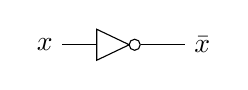
\begin{tikzpicture}
            \node (x) at (0, 1) {$x$};
            \node (y) at (2, 1) {$\bar{x}$};
            \node[not gate US, draw] at ($(x) + (0.8, 0)$) (notx) {};
            \draw (x) -- (notx.input);
            \draw (notx.output) -- ([xshift=0.2cm]notx.output) -- (y);
        \end{tikzpicture}
        \vfill
        \caption*{Not Gate}
    \end{minipage}
    \begin{minipage}[b][2cm][b]{.30\textwidth}
        \centering
        \vfill
        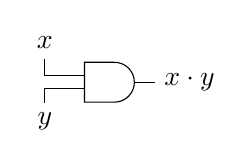
\begin{tikzpicture}
            \node (x) at (0, 0) {$x$};
            \node (y) at (0, -1) {$y$};
            \node[and gate US, draw, rotate=0, logic gate inputs=nn] at ($(x) + (0.8, -0.5)$) (and) {};
            \node[right= 0.25cm of and] (out) {$x\cdot y$};
            \draw (x) |- (and.input 1);
            \draw (y) |- (and.input 2);
            \draw (and.output) -- ([xshift=0.2cm]and.output) -- (out);
        \end{tikzpicture}
        \vfill
        \caption*{And Gate}
    \end{minipage}
    \begin{minipage}[b][2cm][b]{.30\textwidth}
        \centering
        \vfill
        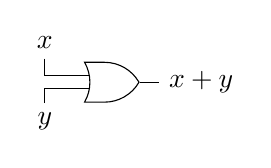
\begin{tikzpicture}
            \node (x) at (0, 0) {$x$};
            \node (y) at (0, -1) {$y$};
            \node[or gate US, draw, rotate=0, logic gate inputs=nn] at ($(x) + (0.8, -0.5)$) (and) {};
            \node[right= 0.25cm of and] (out) {$x+y$};
            \draw (x) |- (and.input 1);
            \draw (y) |- (and.input 2);
            \draw (and.output) -- ([xshift=0.2cm]and.output) -- (out);
        \end{tikzpicture}
        \vfill
        \caption*{Or Gate}
    \end{minipage}
    \begin{minipage}[b][2cm][b]{.30\textwidth}
        \centering
        \vfill
        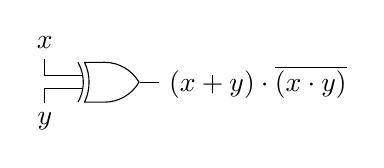
\begin{tikzpicture}
            \node (x) at (0, 0) {$x$};
            \node (y) at (0, -1) {$y$};
            \node[xor gate US, draw, rotate=0, logic gate inputs=nn] at ($(x) + (0.8, -0.5)$) (and) {};
            \node[right= 0.25cm of and] (out) {$(x+y)\cdot\overline{(x\cdot y)}$};
            \draw (x) |- (and.input 1);
            \draw (y) |- (and.input 2);
            \draw (and.output) -- ([xshift=0.2cm]and.output) -- (out);
        \end{tikzpicture}
        \vfill
        \caption*{Xor Gate}
    \end{minipage}
    \begin{minipage}[b][2cm][b]{.30\textwidth}
        \centering
        \vfill
        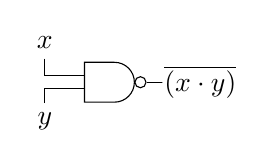
\begin{tikzpicture}
            \node (x) at (0, 0) {$x$};
            \node (y) at (0, -1) {$y$};
            \node[nand gate US, draw, rotate=0, logic gate inputs=nn] at ($(x) + (0.8, -0.5)$) (and) {};
            \node[right= 0.25cm of and] (out) {$\overline{(x\cdot y)}$};
            \draw (x) |- (and.input 1);
            \draw (y) |- (and.input 2);
            \draw (and.output) -- ([xshift=0.2cm]and.output) -- (out);
        \end{tikzpicture}
        \vfill
        \caption*{Nand Gate}
    \end{minipage}
    \begin{minipage}[b][2.5cm][b]{.30\textwidth}
        \centering
        \vfill
        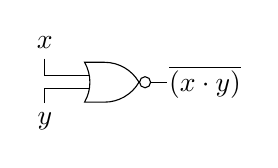
\begin{tikzpicture}
            \node (x) at (0, 0) {$x$};
            \node (y) at (0, -1) {$y$};
            \node[nor gate US, draw, rotate=0, logic gate inputs=nn] at ($(x) + (0.8, -0.5)$) (and) {};
            \node[right= 0.25cm of and] (out) {$\overline{(x\cdot y)}$};
            \draw (x) |- (and.input 1);
            \draw (y) |- (and.input 2);
            \draw (and.output) -- ([xshift=0.2cm]and.output) -- (out);
        \end{tikzpicture}
        \vfill
        \caption*{Nor Gate}\label{}
    \end{minipage}
\end{figure}
These are the basic gates which are used in combinational logic. Using Boolean Algebra, we can simplify complicated logic
statements/circuits.
\begin{center}
    \begin{tabular}{c|c}
     $x\cdot\bar{x} = 0$ & $x+\bar{x}=1$ \\ 
     $x\cdot 0 = 0$ & $x+1=1$ \\  
     $x\cdot 1 = x$ & $x+0=x$ \\ 
     $x\cdot x = x$ & $x+x=x$ \\
     $x\cdot y = y \cdot x$ & $x+y=y+x$ \\
     $(xy)z = x(yz)$ & $(x+y)+z=x+(y+z)$ \\
     $x(y+z)=xy+xz $ & $x+yz=(x+y)(x+z)$ \\
     $xy+x = x $ & $(x+y)x=x$ \\
     $\overline{xy}=\bar{x}+\bar{y} $ & $\overline{x+y}=\bar{x}\bar{y}$ \\
    \end{tabular}
\end{center}
One other important circuit element is the data multiplexor (mux). A mux takes in $n$ different sources of data and selects one of those
sources to output. It does this using select inputs. For example, if a mux has 3 select bits, then it can choose from 8 different streams of data.
\subsection{Timing}
In circuits, timing is incredibly importat because combinational logic blocks have propagation delays (i.e the output does not change instantaneously with the input).
When used in conjuction with registers (which what their own timing requirements), if one is not careful, we could build a circuit which produces inaccurate outputs.
When checking whether or not a circuit will do what it is designed to do, we need to look at two special paths:
\begin{itemize}
    \item Longest CL Path: The longest path of combinational logic blocks between two registers
    \item Shortest CL Path: The shortest path of combinational logic blocks between two registers.
\end{itemize}
This will let us analyze things like the maximum clock rate we can achieve or the maximum hold time our registers can have.
$$t_{delay} = t_{setup}+t_{clk2q}+t_{longestCL}$$
This first formula tells us the maximum amount of time it takes for an input to propagate from a register to another register.
When the clock rises, the first register will read the input and output it $t_{clk2q}$ later. The input will then go through the combinational logic
elements. Since we are looking for the maximum, we only consider the longest CL path. Finally, the output needs to be stable for $t_{setup}$ in order for the
destination register to read it properly. As long as our clock period is longer than the max delay, our circuit will work properly.
$$t_{hold}=t_{clk2q}+t_{shortestCL}$$
This second formula tells us the maximum hold time which our registers can have. When the clock rises, the first register reads the input and outputs it $t_{clk2q}$ later.
The input will then go through the combinational logic elements. Hold time is how long the input needs to be stable after the rising edge of the clock, so if the combinational
logic works incredibly fast, we will need a fast hold time because otherwise the output will change faster than the hold time of the output register. This is why we look at the
shortest CL path. As long as our registers have a hold time which is less than the max-hold, our circuit will work properly.
\section{Datapath}
The processor is the part of the computer which manipulates data and makes decisions. The processor is split into two parts: datapath and control. 
The datapath is the part of the processor with the necessary hardware to perform the operations required by the ISA. THe control tells the datapath what needs to be done.
On every tick of the clock, processors execute a single instruction. Instruction execution takes place in 5 stages.
\begin{itemize}
    \item[1. ] Instruction Fetch
    \item[2. ] Instruction Decode
    \item[3. ] Execute
    \item[4. ] Memory Access
    \item[5. ] Write Back 
\end{itemize}
Each datapath has several main state elements
\begin{itemize}
    \item Register File: An array of registers which the processor uses to keep information out of memory
    \item Program Counter: A special register which keeps track of where the processor is in the program
    \item IMem: A read-only section of memory containing the instructions that need to be executed
    \item DMem: Section of memory which contains data the processor needs to read/write to
\end{itemize}
Important combinational logic elements of the datapath include
\begin{itemize}
    \item Immediate Generator: Generates the immediate
    \item Branch Comparator: Decides whether or not branches should be taken
    \item ALU: Performs mathematical operations
\end{itemize}
All parts of the datapath operate at the same time. The control is how the processor chooses which output to work with.
Control can either be done through combinational logic or by using ROM (Read-Only Memory).
\subsection{Pipelined Datapath}
A single-cycle datapath is one where every instruction passes through the datapath one at a time. However, this is
inefficient because faster stages (such as register reading) are left unused while waiting for slower stages (such as memory reading).
One way to fix this is to pipeline the datapath. This allows multiple instructions to use different parts of the datapath at once, speeding up the
processor because no stage is left unutilized. All we need to do is add registers after each datapath stage. However, this introduces "hazards" into the processor.
\subsubsection{Structural Hazards}
\begin{definition}
    A structural hazard is when two or more instructions compete for access to the same physical resource.
\end{definition}
One solution is to have the instructions take turns to access the resource. The other option is to add more hardware to distribute that resource.
For example, a Regfile structural hazard would be when the processor needs to read registers for one instruction and write a register for another.
This is solved by giving the Regfile two independent read ports and one independent write port. Another example is a memory structural hazard where
instructional memory and data memory are used simultaneously. This is solved by separating them into IMem and DMem.
\subsubsection{Data Hazards}
\begin{definition}
    A data hazard is when two instructions have a data dependency between them
\end{definition}
\textbf{Problem: } One instruction is reading from a register that a previous instruction is writing back to\\
\textbf{Solution: } The WB stage will always update the value first before Instruction Decode reads a new value\\\\
\textbf{Problem: } The result from the ALU will take 2 cycles to be written back. An instruction might need it before then\\
\textbf{Solution 1: } We could stall by introducing no-ops (instructions that do nothing), but this would kill performance.\\
\textbf{Solution 2: } WE can add a loop from the output of the ALU to the ALU input via a mux and add a control element to 
determine when we should use the forwarded value\\\\
\textbf{Problem: } Suppose a load instruction is followed by an instrucction that requires the data loaded from DMEM. The ALU thus needs the data as it is being read. This slot after a load is known as the load delay slot.
If the load delay slot instruction uses the result of the load, then we need to stall for a cycle\\
\textbf{Solution 1: } We could insert a no-op into the code\\
\textbf{Solution 2: } Turn off all write enables and run the second instruction twice
\textbf{Solution 3: } Reorder instructions so that the load delay slot doesn't use the loaded result
\subsubsection{Control Hazards}
\begin{definition}
    A control hazard is when the program flow changes so instructions in the pipeline are no longer relevant
\end{definition}
Notice that this is only a problem when a branch is taken because it means the pipeline must be flushed to get the wrong instructions out of the pipeline (by converting them to no-ops).
A more advanced way to fix this is to implement branch prediction which is where the processor attempts to predict whether or not a branch is taken and load instructions based on that.
\end{document}